\documentclass[]{article}
\usepackage{lmodern}
\usepackage{amssymb,amsmath}
\usepackage{ifxetex,ifluatex}
\usepackage{fixltx2e} % provides \textsubscript
\ifnum 0\ifxetex 1\fi\ifluatex 1\fi=0 % if pdftex
  \usepackage[T1]{fontenc}
  \usepackage[utf8]{inputenc}
\else % if luatex or xelatex
  \ifxetex
    \usepackage{mathspec}
  \else
    \usepackage{fontspec}
  \fi
  \defaultfontfeatures{Ligatures=TeX,Scale=MatchLowercase}
\fi
% use upquote if available, for straight quotes in verbatim environments
\IfFileExists{upquote.sty}{\usepackage{upquote}}{}
% use microtype if available
\IfFileExists{microtype.sty}{%
\usepackage{microtype}
\UseMicrotypeSet[protrusion]{basicmath} % disable protrusion for tt fonts
}{}
\usepackage{hyperref}
\hypersetup{unicode=true,
            pdfborder={0 0 0},
            breaklinks=true}
\urlstyle{same}  % don't use monospace font for urls
\usepackage{graphicx,grffile}
\makeatletter
\def\maxwidth{\ifdim\Gin@nat@width>\linewidth\linewidth\else\Gin@nat@width\fi}
\def\maxheight{\ifdim\Gin@nat@height>\textheight\textheight\else\Gin@nat@height\fi}
\makeatother
% Scale images if necessary, so that they will not overflow the page
% margins by default, and it is still possible to overwrite the defaults
% using explicit options in \includegraphics[width, height, ...]{}
\setkeys{Gin}{width=\maxwidth,height=\maxheight,keepaspectratio}
\IfFileExists{parskip.sty}{%
\usepackage{parskip}
}{% else
\setlength{\parindent}{0pt}
\setlength{\parskip}{6pt plus 2pt minus 1pt}
}
\setlength{\emergencystretch}{3em}  % prevent overfull lines
\providecommand{\tightlist}{%
  \setlength{\itemsep}{0pt}\setlength{\parskip}{0pt}}
\setcounter{secnumdepth}{0}
% Redefines (sub)paragraphs to behave more like sections
\ifx\paragraph\undefined\else
\let\oldparagraph\paragraph
\renewcommand{\paragraph}[1]{\oldparagraph{#1}\mbox{}}
\fi
\ifx\subparagraph\undefined\else
\let\oldsubparagraph\subparagraph
\renewcommand{\subparagraph}[1]{\oldsubparagraph{#1}\mbox{}}
\fi

\date{}

\begin{document}

\subsection{Title}\label{title}

An All-Optical, Non-volatile, Bidirectional,Phase-Change Meta-Switch

\subsection{Authors}\label{authors}

\begin{itemize}
\tightlist
\item
  Mengxin Ren
\item
  Baohua Jia
\item
  Jun-Yu Ou, Eric Plum
\item
  Jianfa Zhang
\item
  Kevin F. MacDonald
\item
  Andrey E. Nikolaenko
\item
  Jingjun Xu
\item
  Min Gu
\item
  Nikolay I. Zheludev
\end{itemize}

\subsection{Abstract}\label{abstract}

\emph{Nanostructured Plasmonic Medium for Terahertz Bandwidth
All-Optical Switching}\\
Using a \emph{nanostructured gold film} to achieve an ultrafast resonant
switch.\\
Based on \emph{Fermi-smearing} and \emph{two photon absorption}.

\subsection{Highlight}\label{highlight}

\textbf{Fermi-smearing:} process in which light absorption at a
frequency $\omega_p$ leads to a non-equilibrium redistribution of electronsnear
the Fermi level (EF). When probed at \(\omega_s\) , this Fermi-smearing
has most impact on transitions between the d-band states lying
\( \Delta E\) = 2.4 eV below the Fermi level to states above the
Fermi level. Fermi-smearing leads to a very strong cubic optical
nonlinearity and nonlinear absorption
(\( \beta \approx 10^{-5} \mathsf{m\,W^{-1}}\)) peaking at a
wavelength of about 516 nm.

\textbf{two-photon absorption:} Direct two-photon absorption takes place
without a real intermediate level as there are no empty states in the
Fermi sea. It occurs through a virtual state when the energy of two
incident photons is combined to bridge a gap that cannot be bridged by
individual photons: $ \hbar \omega_p + \hbar \omega_s > \Delta E$. When
characterized in a pump--probe experiment, the direct two-photon
absorption nonlinearity has a very fast response time because it
requires both the pump \(\omega_p\) and the probe \(\omega_s\) photons
to be present simultaneously, and no slow decay carrier recombination is
involved. In fact the uncertainty principle prescribes a finite lifetime
for the virtual level, and thus a finite nonlinearity response time of
order \( \hbar/\delta E < 1\;\mathsf{fs}\), where
\( \delta E \approx \frac{1}{2} \Delta E\) is the energy difference
between the virtual level and the nearest real state. Even with this
limitation, this is an extremely fast degenerate cubic optical
nonlinearity giving rise to a nonlinear absorption coefficient of order
\( 10^{-8} \mathsf m\,\mathsf W^{-1}\)

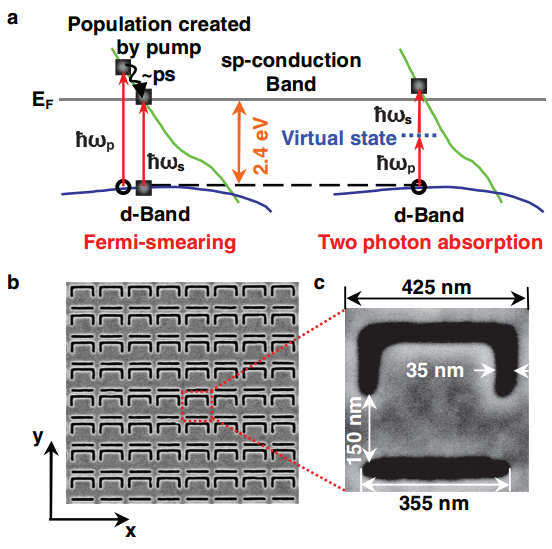
\includegraphics[width=9cm,height=13cm]{image/001_01.png}\\
\textbf{Figure 1.} Metamaterial with giant plasmon-mediated femtosecond
nonlinearity. a) Comparison between Fermi smearing and two-photon
nonlinear responses in gold. b) Scanning electron microscopy (SEM) image
of the nanostructured gold film. c) Detail of a single meta-molecule.

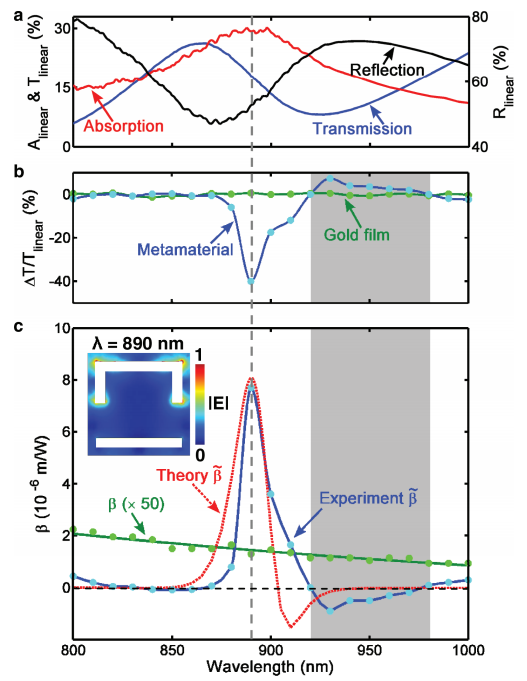
\includegraphics[width=9cm,height=18cm]{image/001_02.png}\\
\textbf{Figure 2.} Metamaterial linear and nonlinear optical properties.
a) Linear absorption, transmission, and reflection spectra of the
metamaterial near its plasmonic resonance. Light is polarized in the
y-direction as defined in Figure 1b. b) Nonlinear transmission change
\( \Delta T/T\) linear at an illumination pulse peak intensity of 2.3
\( \mathsf{GW\,cm^{-2}}\) for the metamaterial and an unstructured
gold reference film. c) The metamaterial's experimentally measured and
theoretically evaluated effective two-photon absorption coefficient
\( \tilde \beta\) compared to that of an unstructured gold film
\( \beta\) (multiplied 50×). The shaded area shows the frequency
range of absorption saturation. The inset shows a numerically simulated
map of the electric field magnitude 10 nm below the gold surface at a
wavelength of 890 nm.

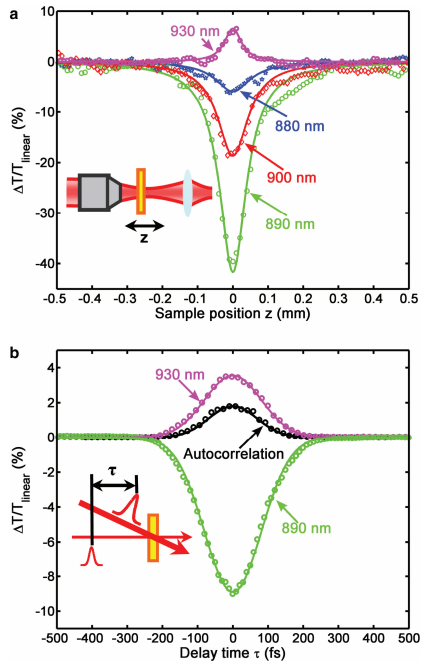
\includegraphics[width=9cm,height=18cm]{image/001_03.png}\\
\textbf{Figure 3.} Giant ultrafast nonlinearity of a plasmonic
metamaterial. a) Z -scan traces taken at an average laser power level of
3 mW (data points) with corresponding analytical fits (lines) for a
selection of characteristic wavelengths near the metamaterial's
plasmonic resonance. b) Time-resolved pump--probe scans showing
nonlinear absorption and bleaching dynamics for the metamaterial
alongside a reference second-harmonic autocorrelation envelope for the
pulses.

\subsection{Related work}\label{related-work}

\end{document}
